\documentclass{icsc}


\usepackage{caption}
\usepackage{subcaption}

\begin{document}

\begin{center}
  \fontsize{14}{20}{\bf Comparison of Electromechanical Means of Stabilizing a
    Bicycle}
\end{center}

%%%%%%%%%%%%%%%% authors %%%%%%%%%%%%%%%
\begin{center}
  \normalsize{\bf{Jason~K.~Moore}}
\end{center}

\begin{center}
  \begin{tabular}{c}
    Faculty of Mechanical Engineering\\
    Delft University of Technology\\
    Mekelweg 2, 2628 CD Delft, The Netherlands\\
    e-mail: j.k.mooore@tudelft.nl\\
  \end{tabular}
\end{center}

\begin{keywords}
  bicycle,
  stability,
  control,
  robot,
  gyroscope,
  ADAS
\end{keywords}

\section{INTRODUCTION}
%
An uncontrolled bicycle can be self-stable at some travel speeds due to the
nature of its design~\cite{Meijaard2007a}. This self-stability relieves the
rider of some of the burden of control and at high speeds riders can balance a
bicycle without much conscious thought. At low speeds, a bicycle becomes more
difficult to control, increasing the chance of falls. It has long been
hypothesized that adding electromechanical sensing and actuation can stabilize
the vehicle relieving some of the human control burden. For safety purposes, I
am interested in systems that share control with the rider but most past work
focus on human independent ``robot riders''.

Van Zytveld~\cite{Zytveld1975} was likely the first to investigate and build a
robot rider for his 1975 Stanford PhD thesis. He used an actuated inverted
pendulum that mimicked rider lean, but was not successful in demonstrating what
his theoretic control model predicted. It was not until the mid 1980s that
someone successfully demonstrated an automatically balanced
motorcycle~\cite{Ruijs1986a}. Ruijs and Pacejka used a steering motor to
stabilize the motion recognizing that simple positive roll rate feedback can
stabilize the vehicle at low speeds, i.e. ``steer into the direction of roll
motion''.
% This same approach was used by the 2005 DARPA challenge vehicle Ghostrider~\cite{todo}.
In 2005, the Murata Manufacturing company demonstrated ``Murata Boy'', a
bicycle robot which utilized a reaction wheel capable of generating stabilizing
roll torques~\cite{WikipediaAuthors2023}. In 2006, several Dartmouth University
undergraduates developed a simple motor driven flywheel encased in the front
wheel that increases the front wheel spin momentum providing a roll motion
stabilizing effect~\cite{Ward2006}. This application used the same principle as
the rear wheel flywheel of the 1921 Giesberger Gyrocar~\cite{Self2023}. In
2013, Lit Motors~Inc. demonstrated a pair of control moment gyros capable of
balancing a two seater enclosed motorcycle at low speed that used the same
principle used in Brennan's 1903 Gyro
monorail~\cite{WikipediaGyromonorail2012}. There have been numerous other
theoretical and realized machines that utilize one or more of these five
actuation methods throughout the years.

With over a century of innovations in automatically stabilizing single track
vehicles, nothing has ever become commercially viable or demonstrated enhanced
rider or passenger safety. In this study, I will describe how each of these
roll stabilization methods work, what their advantages and disadvantages are,
and discuss whether they can be useful for bicycle safety.

\section{STEER MOTOR SYSTEM}
%
As an example for this abstract, I will demonstrate roll and steer motion
stabilization using an ideal motor actuator that applies equal and opposite
torque to the steered frame from the ridden frame; same as \cite{Ruijs1986a}. I
start by assuming that the bicycle's basic state (steer and roll configuration
and motion) can be accurately measured by using inertial measurement units and
state estimation. The bicycle dynamics model is based on the linearized
Carvallo-Whipple model from \cite{Meijaard2007a} but populated with more
realistic numerical parameters. By assuming full state feedback, the system can
be modeled by these linear state space equations:
%
\begin{align}
  \dot{\bar{x}} = \left( \mathbf{A} - \mathbf{B} \mathbf{K} \right) \bar{x} + \mathbf{B} \bar{u}
\end{align}

\(\mathbf{A}\) represents the passive dynamics of bicycle and \(\mathbf{B}\)
gives the input dynamics from the rider or steer motor applied steering torque.
Full state feedback can be used to drive the steering motor torque
\(T_{\delta,m}=-\mathbf{K}\bar{x}\), giving the closed loop dynamics
\(\mathbf{A} - \mathbf{B} \mathbf{K}\). The state and input vectors are:
%
\begin{align}
  \bar{x} =
    \begin{bmatrix}
      \phi \\
      \dot{\phi} \\
      \delta \\
      \dot{\delta}
    \end{bmatrix} =
    \begin{bmatrix}
      \textrm{roll angle} \\
      \textrm{roll rate} \\
      \textrm{steer angle} \\
      \textrm{steer rate}
    \end{bmatrix}
  \textrm{ and }
  \bar{u} =
    \begin{bmatrix}
      T_{\delta} \\
    \end{bmatrix} =
    \begin{bmatrix}
      \textrm{rider applied steer torque} \\
    \end{bmatrix}
\end{align}
%
\begin{figure}
  \centering
  \begin{subfigure}{0.49\textwidth}
    \centering
    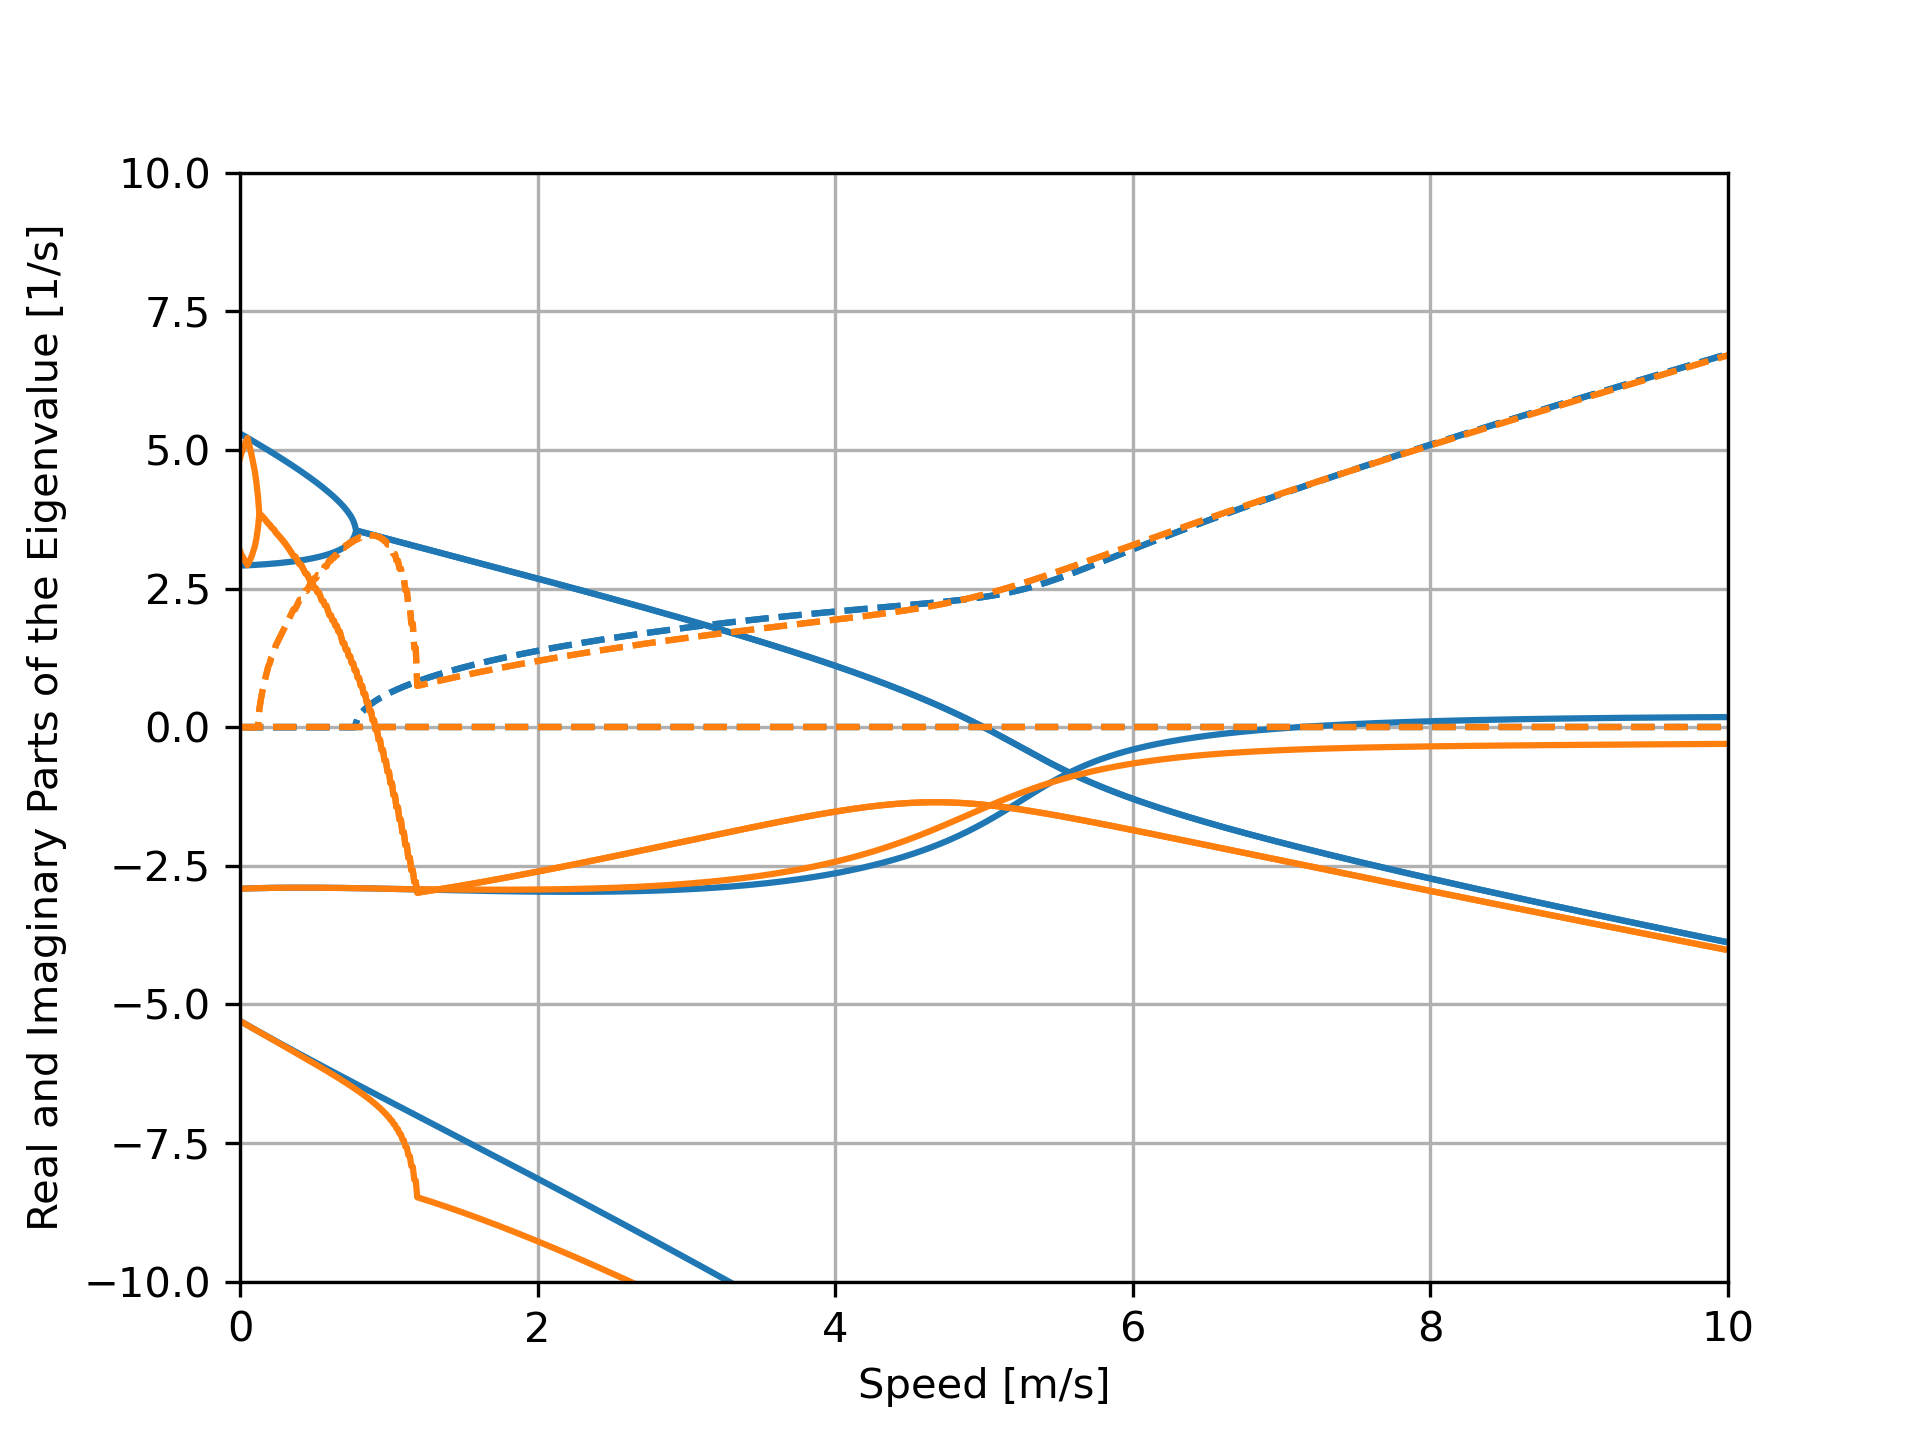
\includegraphics[width=\textwidth]{lqr-eig.png}
    \caption{Root locus of eigenvalue components with the LQR gain scheduling
      across speed.
      Blue lines are the passive bicycle dynamics and orange are the
      automatically controlled dynamics. Solid lines are real parts and dotted
      lines are imaginary parts.}
    \label{fig:lqr-eig}
  \end{subfigure}
  \hfill
  \begin{subfigure}{0.49\textwidth}
    \centering
    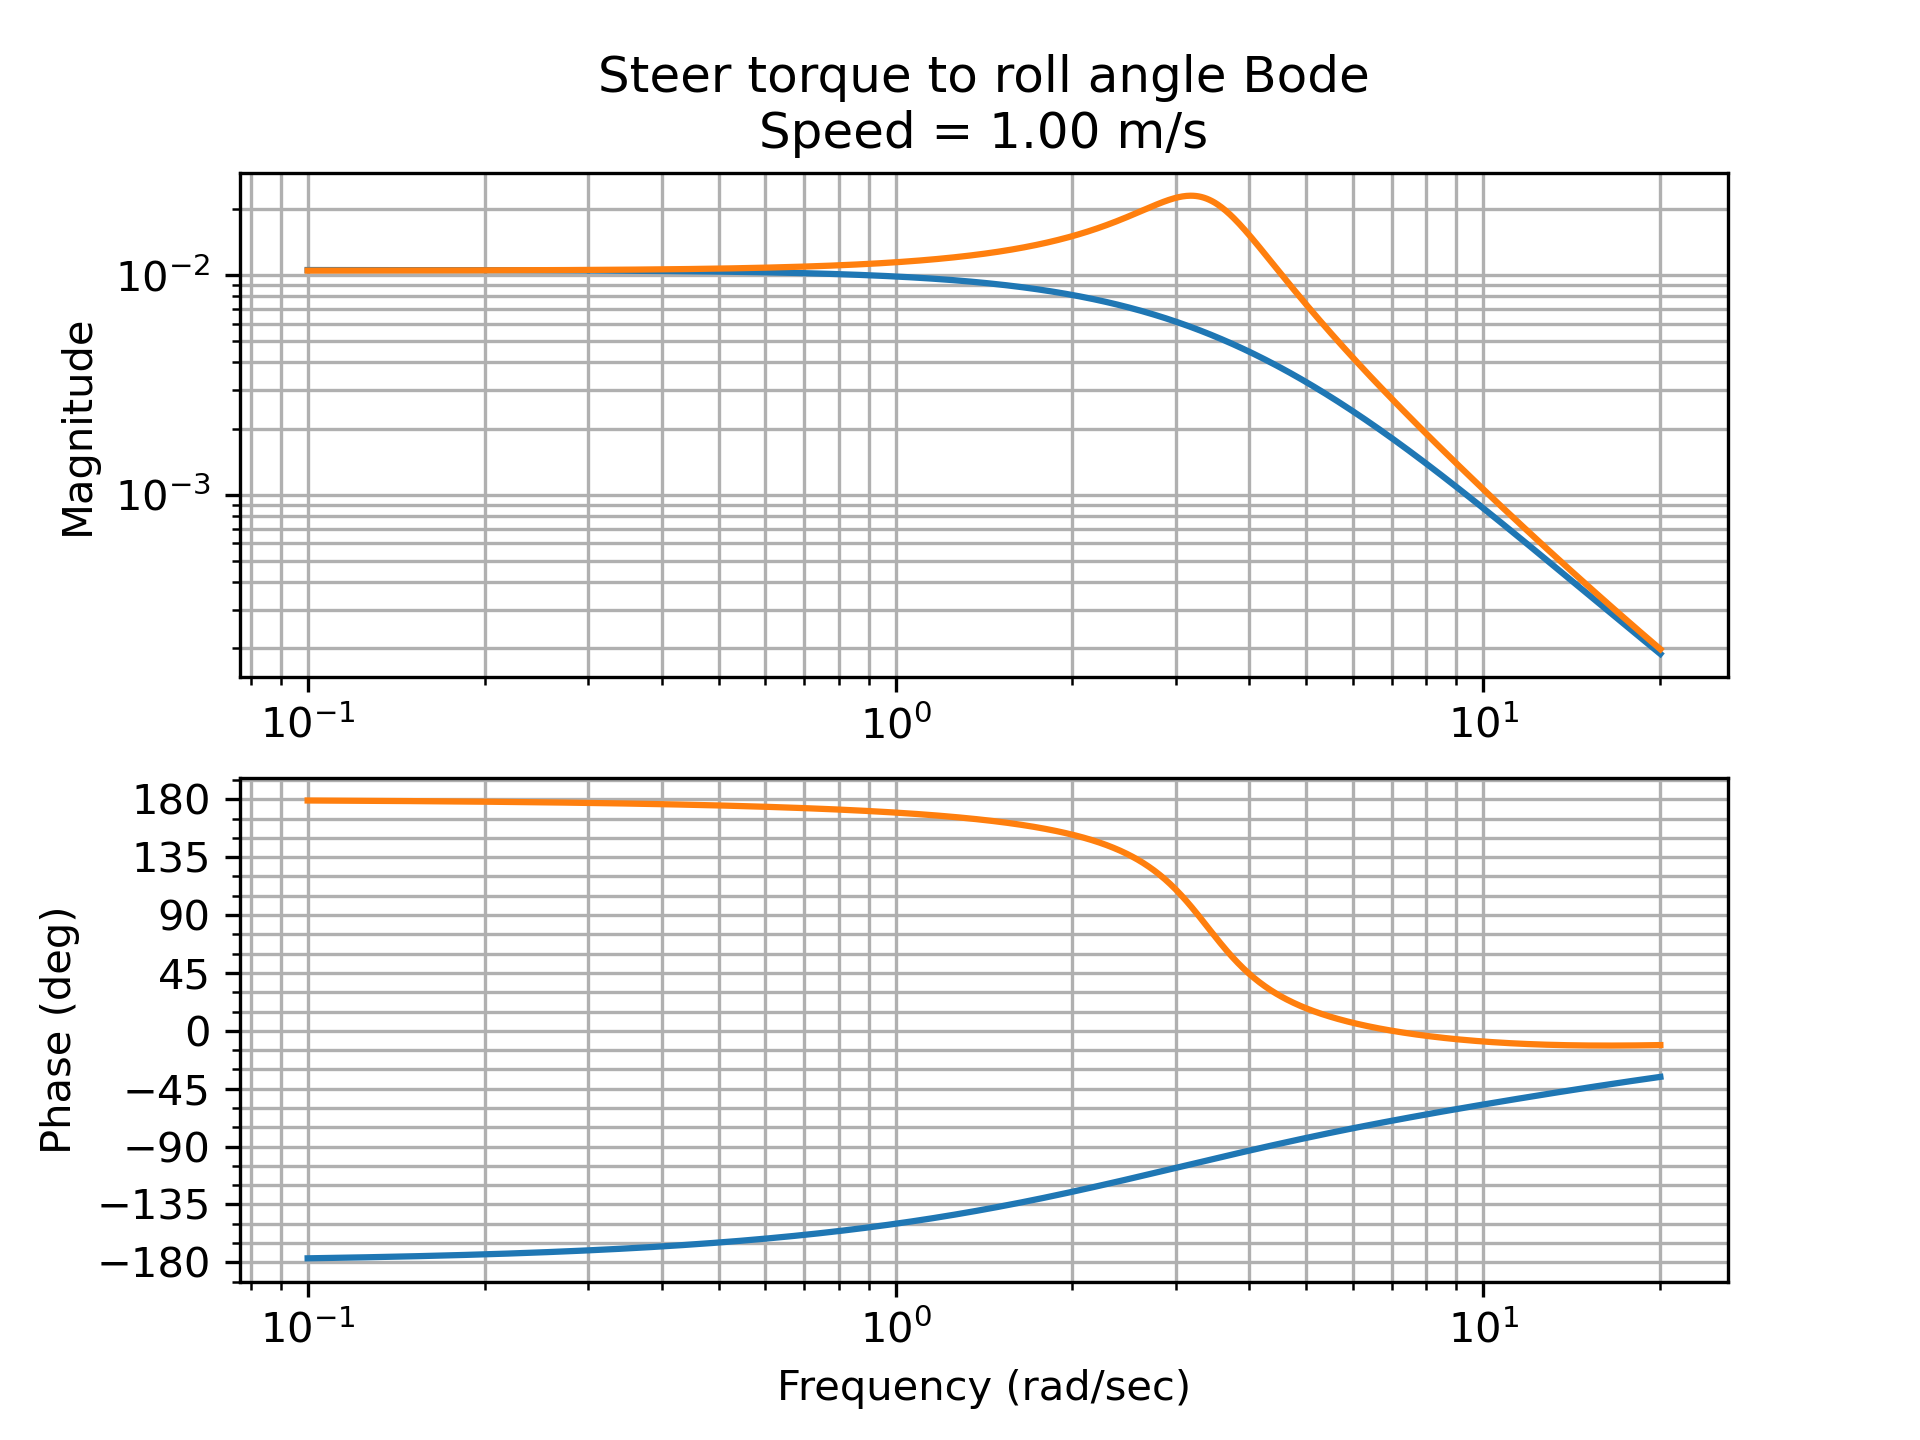
\includegraphics[width=\textwidth]{lqr-steer-roll-bode-compare-v01.png}
    \caption{Bode plots for rider applied steer to roll dynamics for the
      uncontrolled bicycle (blue) and automatically controlled bicycle
      (orange).}
    \label{fig:bode}
  \end{subfigure}
  \caption{Uncontrolled and controlled dynamics.}
\end{figure}

By applying a maximum torque scaled linear quadratic regulator (LQR) across all
speeds the scheduled feedback gains \(\mathbf{K}\) can be found to stabilize
the vehicle at almost all speeds with minimal effect to the dynamics of the
vehicle besides the positive aspect of stabilization, similar to
\cite{Schwab2008}. Figure~\ref{fig:lqr-eig} shows that the bicycle can be
stabilized down to 1 m/s and that the natural frequencies and time constants do
not change drastically, leaving the bicycle's dynamics intact. It is also
important to note that from the rider's perspective \(\mathbf{A} - \mathbf{B}
\mathbf{K}\) is simply a new plant they must control, yet through the same
passive input filter which is a function of the unchanged \(\mathbf{B}\) matrix
governing the rider's steer input. Figure~\ref{fig:bode} shows that at 1 m/s
the rider will experience a less damped response to steering in the 0.3 to 0.8
Hz bandwidth, so the handling is not necessarily maintained when applying
automatic control. To keep the handling the same, more elaborate model
reference control would be required.

\section{CONCLUSIONS}
%
In the presentation, I will share similar analyses for a moving mass actuator,
paired control moment gyros, reaction wheel, and front wheel internal flywheel
and show how most are equivalent ways of achieving the same goal. I will then
compare them for feasibility and effectiveness. This will be presented in a
both historical and modern context of realized vehicles and why the vehicles
may or may not be able to enhance safety and be commercially viable.

\bibliographystyle{plain}
\bibliography{ICSC2023}

\end{document}

